\documentclass{article}
\usepackage[utf8]{inputenc}
\usepackage{float}
\usepackage{graphicx}
 
\title{Tugas 1 Pemrograman 2}
\author{Oleh\\Ahmad Agung Tawakkal\\
1184015\\
D4 TI 2B}
\date{October 2019}
 
\graphicspath{{Images/}}
 
\begin{document}
 
\maketitle

\newpage

\section {Sejarah Python}

    \paragraph{}Bahasa Pemrograman python ada pada tahun 1980 oleh Guido van Rossum di CWI Belanda. Van Rossum  adalah penulis utama Python, kemudian pada tahun 2000 python merilis versi 2.0 dangan memiliki banyak fitur yang baru, seperti cycle-detecting garbage collector untuk mengotomasi manajemen memori. Versi 2.0 dinilai lebih transparan dan inklusif untuk pengembangan software ketimbang versi sebelumnya. Hal ini didukung dengan adanya PEP – Python Enhancement Proposal, sebuah spesifikasi teknis yang menjadi tuntunan informasi untuk penggunanya dan menggambarkan fitur baru pada Python.\\
    
    \par Python versi 3.0 adalah versi dengan banyak perubahan, termasuk memasukkan statemen print ke dalam built-in function. Python vesi 3.0 dirilis pada akhir tahun 2008. Python 2.7 dirilis pada tahun 2010 yang bertujuan agar pengguna python versi 2 mudah berpindah ke python versi 3.\\
    
    \subsection{Implementasi dan Penggunaan Python pada Perusahaan}
        \paragraph{}Implementasi penggunaan python pada perusahaan adalah sebagai berikut :
            \begin{enumerate}
                \item Ketersediaan akan open-source library, frameworks, tools untuk data mining, contohnya adalah SciKit Learn, TensorFlow, Keras.
                \item Relatif lebih mudah dipahami. Penulisan code di Python relatif lebih singkat.
                 \item Multifungsi, tidak hanya untuk data processing, namun juga bisa untuk tugas lain seperti membuat website dan tampilan GUI (Graphical User Interface).
            \end{enumerate}
            
\section{Instalasi}
    \subsection{Instalasi Python 3}
        \begin{enumerate}
            \item Download python sesuai dengan OS yang di pakai, anda dapat mengunduh di https://www.python.org/downloads/release/python-370.
            \item Kemudian Klik 2x pada file instalasi python.
            \item Pilih Install Now.
            \item Tunggu hingga selesai Instalasinya.
        \end{enumerate}

\subsection{Instalasi PIP}
    \begin{enumerate} 
        \item Download PIP sesuai dengan versi python yang di pakai, anda dapat mengunduh PIP di https://pypi.org/project/pip/files.
        \item Kemudian klik 2 kali pada get-pip.py atau setup.
        \item Kemudian masuk ke Control Panel - System And Security - System - Advanced System Settings
        \item Lalu klik Environment Variables, pada sesi System Variables pilih path - Edit - New - C:/Python3.7/Scripts - Ok.
        \item Buka Command Prompt, kemudian ketik PIP.
        \item Selesai
    \end{enumerate}
    
\subsection{Setting Environment}
    \begin{enumerate} 
        \item Masuk ke Control Panel - System And Security - System - Advanced System Settings
         \item Lalu klik Environment Variables, pada sesi System Variables pilih path - Edit - New - C:/Python3/Scripts - Ok.
    \end{enumerate}

\subsection{Mencoba entrepriter/CLI pada terminal atau cmd}
    \begin{enumerate}
        \item Buka terninal atau cmd.
        \item Ketik python pada cmd atau terminal.
        \item Kemudian untuk print sebuah text anda tinggal menambahkan text print ("Hello word!").
    \end{enumerate}


\subsection{Menjalankan dan mengupdate Anaconda dan Spyder}
    \begin{enumerate}
        \item Dowonload anaconda di https://www.anaconda.com/distribution.
        \item Install anaconda.
        \item Jika sudah di install, selanjutnya lansung buka anacondanya dengan mengklik 2x.
        \item Pada menu utama aplikasi anaconda maka akan terdapat beberapa tools yang disediakan, termasuk spyder dan lain-lain.
        \item Untuk mengupadate, pertama anda harus buka anaconda, kemudaian Environment - Klik tombol play pada base root - kemudian pilih terminal.
        \item Setelah membuka terminal anda ketik perintah "conda update -n dspyr --all" , kemudian akan muncul perintah apakah anda akan mengupadete atau tidak (y/n).
\end{enumerate}

\subsection{Cara Menjalangkan Script Hello Word di spyder} 
    \begin{enumerate}
        \item Pertama anda membuka aplikasi spyder, kemudian tambahkan scrip seperti pada gambar berikut.
        \item Kemdian Klik tombol play untuk menjalankan programnya.
        \item Selanjutnya maka akan muncul di layar console, kemudian akan ada perintah untuk menyapa, misalkan pada gambar dibawah, saya menyapa nama yang bernama agung,maka akan menampilkan "Hello agung", begitu juga dengan Hello Word pada figure 2.
        \begin{figure}
           \begin{center}
                  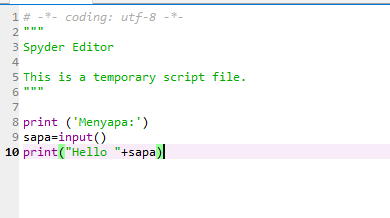
\includegraphics[width=8cm]{gambar1.jpg}
                  \caption{Script untuk menampilkan text string Hello dan inputan user}
            \end{center}
        \end{figure}
        \begin{figure}    
            \begin{center}
                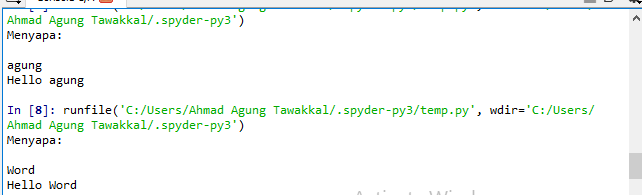
\includegraphics[width=8cm]{gambar2.PNG}
                \caption{Hasil inputan user}
            \end{center}
        \end{figure}      
    \end{enumerate}

\newpage

\subsection{Menjalangkan script login otomatis dengan library selenium dan inputan user} 
    \begin{enumerate}
        \item Pertama anda membuka Command Prompt.
        \item Untuk instal selenium tambahkan text "pip install selenium".
        \item Tunggu hingga selesai.
        \item Selanjutnya anda harus mengecek versi dari web browser anda.
        \item Kemudian anda download driver dari browser yang anda gunakan.
        \item Setelah download drivernya, tempelkan file drivernya di "C:\Windows\System32".
        \item Kemduian buka spyder dan tambahkan codingan seperti pada Figure 3.
            \begin{figure}[H]
                \centerline{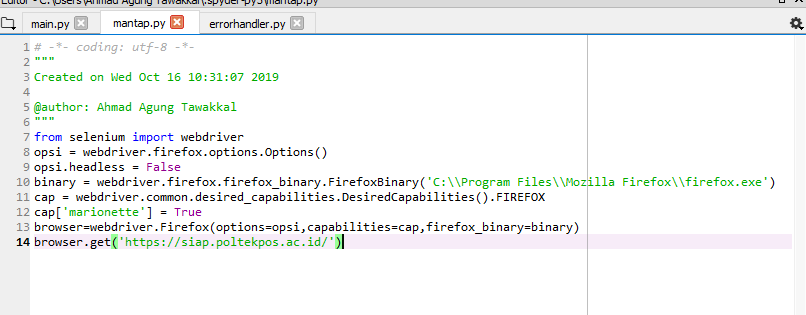
\includegraphics[width=10cm]{gambar6.PNG}}
                \caption{}
            \end{figure}
        \item Pada line 10 yang diberi tanda dalam kurun, kemudian sesuaikan dengan tempat instalasi file browser yang anda gunakan. Pada line ke 14 yang tanda kurung adalah alamat web site yang akan dibuka.
        \item setelah selesai anda dapat Run programnya atau dengan menekan tombol F5 pada keyboar laptop.
        \item Setelah di Run maka browser akan login otomatis ke halaman web yang dituju.
    \end{enumerate}

\subsection{Cara menggunakan variable explorer pada spyder}
    \begin{enumerate}
        \item Buka spyder.
        \item Kemudian pada progam anda tambahkan variabel a yang berisi integer yang nilainya 1 kemudian variable b berisi iteger juga yang nulainya 3.
        \item Variable c menjumlahkan variable a dan b, c=a+b.
        \item Pada tampilan variable explorer maka akan terlihat secara jelas nilai dari a dan b serta menghitung jumlah nilai dari hasil penjumlahan yang ditampung di variable c.
    \end{enumerate}

\section{Identasi}

\subsection{Penjelasan Identasi}
    \begin{enumerate}
        \item Indentasi adalah penambahkan spasi pada awal baris-baris program agar program mudah dibaca.
    \end{enumerate}

\subsection{Jenis eror identasi yang ditemukan} 
    \begin{enumerate}
        \item Identasi IF.
        \item Identasi Else.
        \item Identasi Elif.
            \begin{figure}[ht]
                \centerline{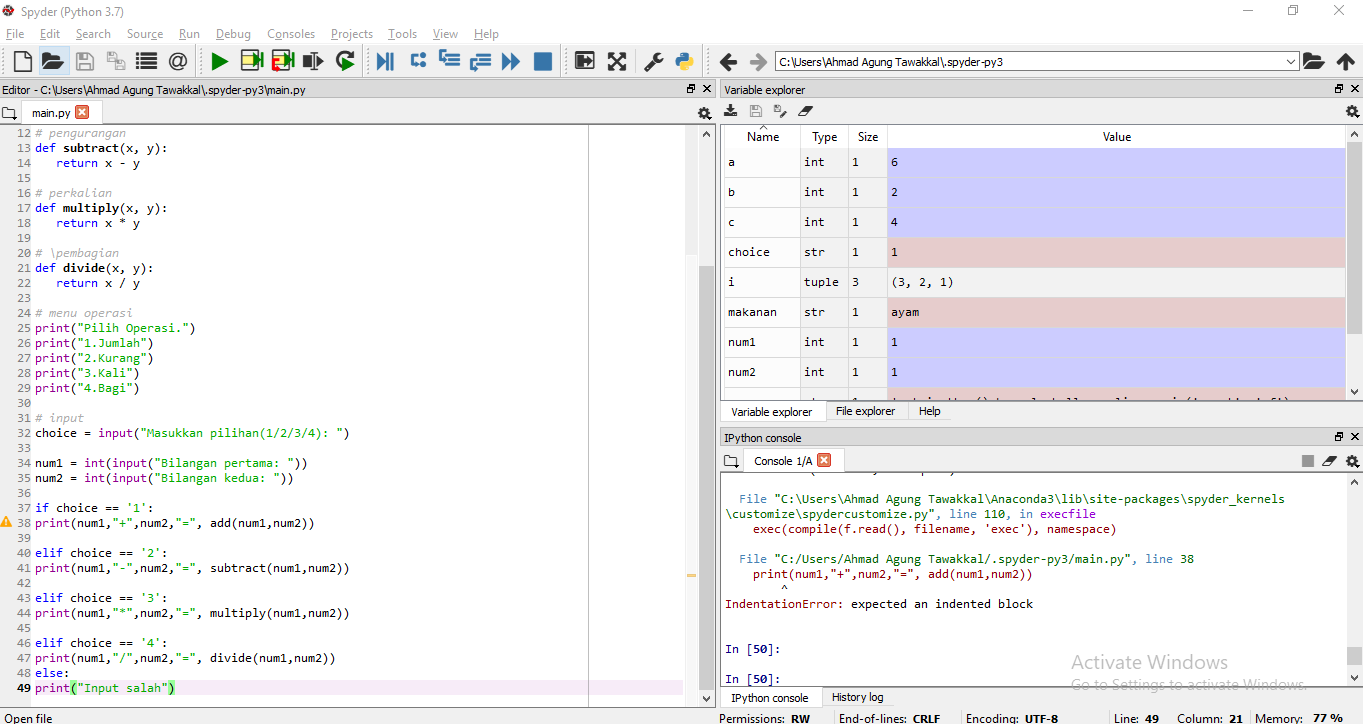
\includegraphics[width=7cm]{gambar3.PNG}}
                \caption{Contoh error}
            \end{figure}
            \begin{figure}[ht]
                \centerline{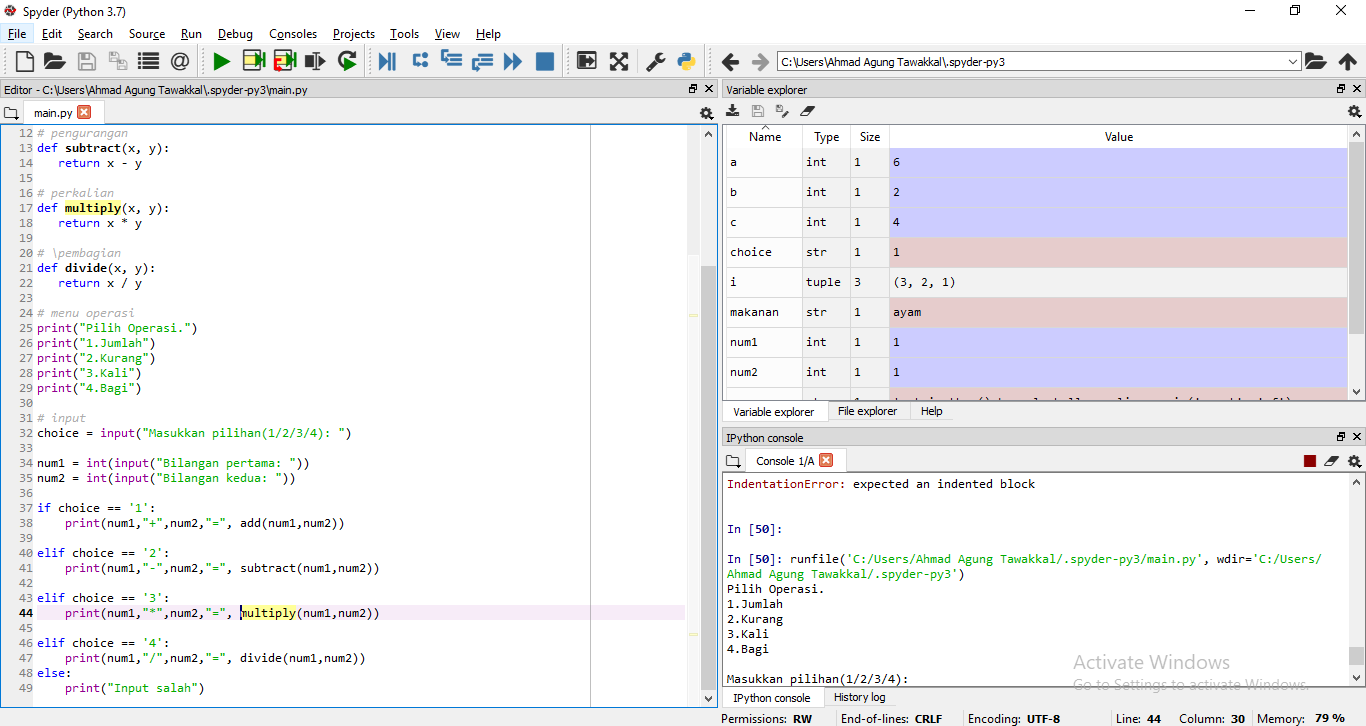
\includegraphics[width=7cm]{gambar4.PNG}}
                \caption{Contoh benar}
            \end{figure}
                \paragraph{}Ketika program yang if, else, dan elif tidak diberi spasi bagian awalannya makan akan error seperti gambar diatas. Sedangkan jika diberi spasi pada awal, maka programnya akan benar.
                
    \end{enumerate}
    
\subsection {Cara membaca eror}
    \begin{enumerate}
        \item Pertama anda harus melihat layar konsolnya.
        \item Kemudian akan menampilkan bagian mana yang salah, seperti pada contoh berikut.
            \begin{figure}[ht]
                \centerline{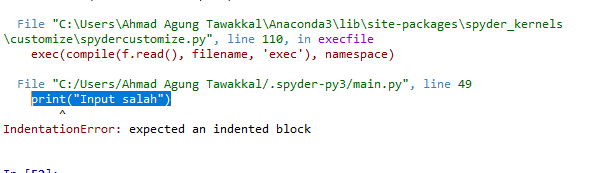
\includegraphics[width=10cm]{gambar5.PNG}}
                \caption{Mencari bagian yang error}
            \end{figure}
                \paragraph{}Pada gambar diatas memperlihatkan bagian yang error pada program yang dibuat.
    \end{enumerate}
    
\subsection {Cara menangani eror}
    \begin{enumerate}
        \item Untuk menengani error tinggal melihat errornya apa dan melihat bagian line keberapa yang error seperti pada gambar yang diatas, yang memiliki error di line 49.
        \item Jika masih error anda dapat mencari solusi di internet atau konsultasi ke dosen maupun teman.
    \end{enumerate}

\section{Presentasi Tugas}
\paragraph{}https://www.youtube.com/watch?v=xd0bPoB1JiA&feature=youtu.be



\end{document}

